\documentclass{beamer}
\usepackage[utf8]{inputenc}
  
\usetheme{Madrid}
\usecolortheme{default}
\usepackage{amsmath,amssymb,amsfonts,amsthm}
\usepackage{txfonts}
\usepackage{tkz-euclide}
\usepackage{listings}
\usepackage{adjustbox}
\usepackage{array}
\usepackage{tabularx}
\usepackage{gvv}
\usepackage{lmodern}
\usepackage{circuitikz}
\usepackage{tikz}
\usepackage{graphicx}
\usepackage[T1]{fontenc}
\UseRawInputEncoding

\setbeamertemplate{page number in head/foot}[totalframenumber]

\usepackage{tcolorbox}
\tcbuselibrary{minted,breakable,xparse,skins}



\definecolor{bg}{gray}{0.95}
\DeclareTCBListing{mintedbox}{O{}m!O{}}{%
  breakable=true,
  listing engine=minted,
  listing only,
  minted language=#2,
  minted style=default,
  minted options={%
    linenos,
    gobble=0,
    breaklines=true,
    breakafter=,,
    fontsize=\small,
    numbersep=8pt,
    #1},
  boxsep=0pt,
  left skip=0pt,
  right skip=0pt,
  left=25pt,
  right=0pt,
  top=3pt,
  bottom=3pt,
  arc=5pt,
  leftrule=0pt,
  rightrule=0pt,
  bottomrule=2pt,
  toprule=2pt,
  colback=bg,
  colframe=orange!70,
  enhanced,
  overlay={%
    \begin{tcbclipinterior}
    \fill[orange!20!white] (frame.south west) rectangle ([xshift=20pt]frame.north west);
    \end{tcbclipinterior}},
  #3,
}
\lstset{
    language=C,
    basicstyle=\ttfamily\small,
    keywordstyle=\color{blue},
    stringstyle=\color{orange},
    commentstyle=\color{green!60!black},
    numbers=left,
    numberstyle=\tiny\color{gray},
    breaklines=true,
    showstringspaces=false,
}



\title 
{MatGeo Assignment 1.2.13}

\author
{AI25BTECH11007}
\begin{document}

\frame{\titlepage}
\begin{frame}{Question}
Construct a triangle $ABC$ in which 
\[
BC = 5 \,\text{cm}, \quad\angle B = 45^\circ, \quad \text{and} \quad AC + AB = 7.5 \,\text{cm}.
\]

\end{frame}

\begin{frame}{Solution}
     Using the cosine formula in $\triangle ABC$,
\begin{align}
b^{2} &= a^{2} + c^{2} - 2ac\cos B \\
\Rightarrow (7.5-c)^{2} &= 5^{2} + c^{2} - 2\cdot 5c \cos 60^\circ \\
\Rightarrow c &= \frac{7.5^{2}-5^{2}}{2(7.5-5\cos 60^\circ)} 
\end{align}

\[
c = 3.125, 
\qquad b = 7.5 - 3.125 = 4.375.
\]

\[
A=\myvec{\tfrac{3.125\cos 60^\circ}{\sin 60^\circ}\\[6pt]\tfrac{3.125}{\sin 60^\circ}},\quad 
B=\myvec{0\\0},\quad 
C=\myvec{5\\0}.
\]
\end{frame}

\begin{frame}{Solution}
The coordinates of $\triangle ABC$ are
\[
A=\myvec{\tfrac{3.125}{\sqrt{3}} \\[6pt] \tfrac{6.25}{\sqrt{3}}}
\;\approx\;
\myvec{1.804 \\[6pt] 3.608},\quad
B=\myvec{0 \\ 0},\quad
C=\myvec{5 \\ 0}.
\]
\end{frame}

\begin{frame}{Construction Plot}
\begin{figure}
    \centering
    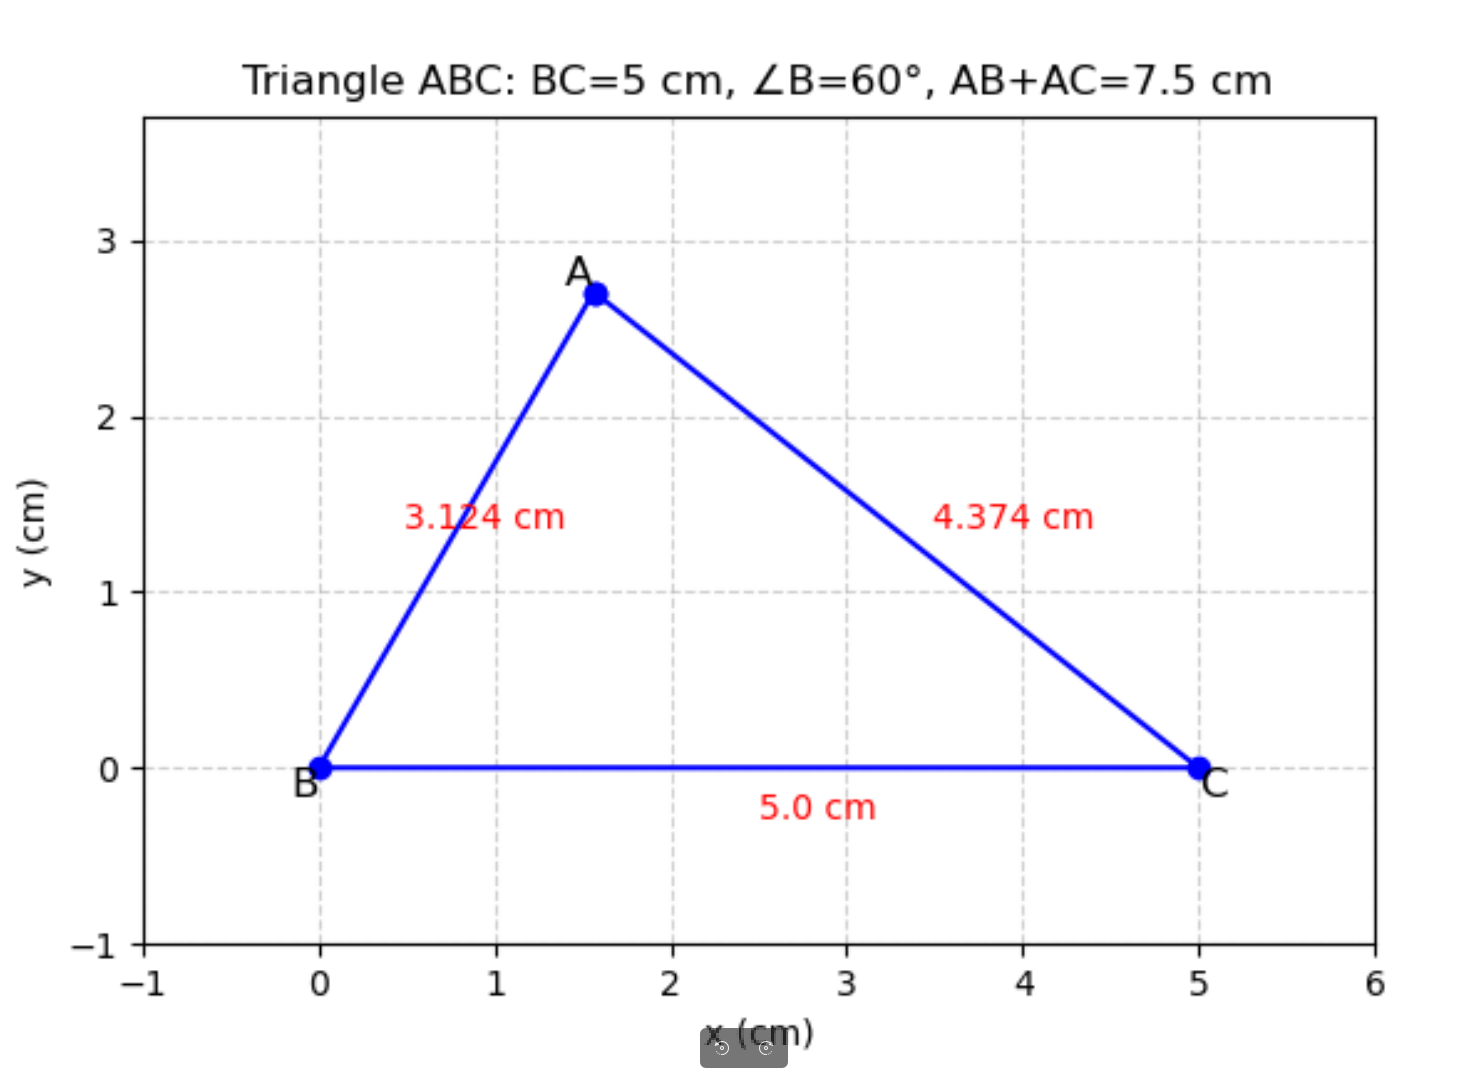
\includegraphics[width=1\linewidth]{figs/image.png}
    \caption{Construction Plot}
    \label{fig:figs/image.png}
\end{figure}
\end{frame}


\begin{frame}[fragile]{C Code: Dot Product and Magnitude}
\begin{lstlisting}[language=C]
#include <stdio.h>
#include <math.h>

int main(void) {
    /* Given data */
    double a = 5.0;       /* BC */
    double K = 7.5;       /* AC + AB = b + c */
    double cosB = 0.5;    /* cos 60° */
    double sinB = sqrt(3.0) / 2.0; /* sin 60° */

    /* Formula from your solution */
    double c = (K*K - a*a) / (2.0 * (K - a * cosB));
    double b = K - c;

    /* Coordinates with B=(0,0), C=(a,0) */
    double Ax = (c * cosB) / sinB;
    double Ay = c / sinB;

    

\end{lstlisting}
\end{frame}

% C code part 2
\begin{frame}[fragile]{C Code: Angle Calculation and Main}
\begin{lstlisting}[language=C]
printf("Computed values:\n");
    printf("c (AC) = %.6f\n", c);
    printf("b (AB) = %.6f\n", b);
    printf("A = (%.6f, %.6f)\n", Ax, Ay);
    printf("B = (0.000000, 0.000000)\n");
    printf("C = (%.6f, 0.000000)\n", a);

    return 0;
}
\end{lstlisting}
\end{frame}

 


% Python code part 1
\begin{frame}[fragile]{Python Code: Setup and Points}
\begin{lstlisting}[language=Python]
import matplotlib.pyplot as plt
import numpy as np

# Coordinates of vertices
A = np.array([1.5625, 2.705])   # Computed intersection
B = np.array([0, 0])            # Origin
C = np.array([5, 0])            # On x-axis
\end{lstlisting}
\end{frame}

% Python code part 2
\begin{frame}[fragile]{Python Code: Plot Triangle}
\begin{lstlisting}[language=Python]
fig, ax = plt.subplots()

# Plot the triangle edges
triangle_points = np.array([A, B, C, A])
ax.plot(triangle_points[:, 0], triangle_points[:, 1], 'b-', marker='o')

# Annotate vertices
ax.text(A[0], A[1], 'A', fontsize=12, ha='right', va='bottom')
ax.text(B[0], B[1], 'B', fontsize=12, ha='right', va='top')
ax.text(C[0], C[1], 'C', fontsize=12, ha='left', va='top')
\end{lstlisting}
\end{frame}

% Python code part 3
\begin{frame}[fragile]{Python Code: Final Touches and Save}
\begin{lstlisting}[language=Python]
# Formatting and labels
ax.set_aspect('equal', 'box')
ax.grid(True, linestyle='--', alpha=0.6)
ax.set_xlabel('x (cm)')
ax.set_ylabel('y (cm)')
ax.set_title('Triangle ABC: BC=5 cm, ∠B=60°, AB+AC=7.5 cm')

# Axis limits with padding
padding = 1
min_x, max_x = min(A[0], B[0], C[0]) - padding, max(A[0], B[0], C[0]) + padding
min_y, max_y = min(A[1], B[1], C[1]) - padding, max(A[1], B[1], C[1]) + padding
ax.set_xlim(min_x, max_x)
ax.set_ylim(min_y, max_y)

# Save and display
plt.savefig('triangle_plot.png', dpi=300)
plt.show()
\end{lstlisting}
\end{frame}
\end{document}